\documentclass[fleqn,10pt]{wlpeerj}
\title{Simulation of Brain Functional Connectivity on Empirical and Randomized Brain Structural Networks}

\author[1]{\c{S}eyma \textsc{Bayrak}}
\author[2,3]{Vesna \textsc{Vuksanovi\'c}}
\author[2,3]{Philipp \textsc{H\"{o}vel}}

\affil[1]{Institute of Biology, Otto-von-Guericke-Universit{\"a}t Magdeburg, Leipziger Straße 44, 39120 Magdeburg, Germany}
\affil[2]{Institut f{\"u}r Theoretische Physik, Technische Universit\"at
Berlin, Hardenbergstra\ss{}e 36, 10623 Berlin, Germany }
\affil[3]{Bernstein Center for Computational Neuroscience, Humboldt-Universit{\"a}t zu Berlin, Philippstra{\ss}e 13, 10115 Berlin, Germany }


\keywords{resting-state, functional and anatomical connectivity, time-delayed oscillations, hemodynamic model, network science}

\begin{abstract}
Blood oxygen level dependent (BOLD) contrast imaging is one of the widely used fMRI techniques to map the brain activity at resting-state, i.e. in the absence of any stimulus-driven task.  The BOLD fluctuations arising from changing neuronal activity at resting-state have been observed to be complex but highly structured and robust. A well-explored BOLD response in the brain would potentially lead to easier diagnosis of neurodegenerative disorders such as Alzheimer's disease and Parkinson's disease. However, the underlying biophysical mechanism of the resting-state activity of the brain has not yet been completely uncovered. This study combines experimental and modeling approaches in order to investigate the temporal and structural dynamics of the human brain at resting-state. The temporal dynamics of the neuronal activity is modeled with FitzHugh-Nagumo neuronal oscillators and BOLD activity is inferred via the  Balloon-Windkessel hemodynamic model. It is aimed to \textit{i)} investigate the network topology of structural connectivity by comparing it to random graphs, \textit{ii)} demonstrate  how functionally correlated BOLD signals would emerge from the anatomical connections, and \textit{iii)} explore whether or not the modeled temporal dynamics on brain networks is distinguishable than that of its randomized networks.


\end{abstract}

\begin{document}

\flushbottom
\maketitle
\thispagestyle{empty}





\section*{Introduction}


Large-scale functional brain connectivity maps are networks of brain regions based on functional interactions, i.e. any co-activation between these regions \citep{BIS95, BRE10b, DAM06}. In a typical fMRI experiment,  functional connections are obtained from brain regions, whose corresponding time-series of blood-oxygen-level-dependent (BOLD) activity display significant correlations at low-frequencies ($< 0.1$ Hz). Well organized spatio-temporal low-frequency fluctuations have been reported in BOLD-fMRI signals of a mammalian brain at resting-state, i.e. under no simulation and in the absence of any simulation-driven task. \citep{BIS95, DAM06, VIN07a}.  Despite important progress over the past few years, the way how functional connectivity arises from the complex anatomical connectivity still remains poorly understood \citep{GHO08, DEC09, CAB12, CAB14, VUK14}.

Existing models of resting-brain dynamics hypothesize that functional interactions result from a complex interplay between intrinsic brain dynamics and underlying structural connections \citep{HAG08, GHO08, RUB09, DEC12, VUK13}. Previously, the neuronal dynamics have been modeled as coupled non-linear oscillators \citep{WIE61, LOP97, NUN98, NUN00, PO08}, Hopf oscillators \citep{JIR07}, Wilson-Cowan systems \citep{DEC09}, FitzHugh-Nagumo systems \citep{GHO08, VUK13} and Kuromoto oscillations \citep{BRE10i, VUK14}. In particular, these models explore the range of conditions at which functional networks emerge from anatomical connections: the role of multiple time-scales in the formation of functional connectivity networks \citep{HON07}, time delays in the signal propagation between the network nodes as well as the system noise \citep{GHO08, GHO08a}, local network oscillations \citep{DEC09, CAB11} and structural disconnection \citep{CAB12}.

Our investigations provide a deeper insight to the relation between functional and anatomical brain connectivity: how the non-random dynamical process of brain's functional connectivity could be shaped by its structural topology. The networks are constructed on resting-state anatomical connectivity (AC) map via binarization at varying connection probabilities $p$. We also construct random networks by manipulating AC map via Erd\H{o}s-R\'{e}nyi tool \citep{XYZERD}. The neuronal activity and the BOLD fluctuations are simulated on both network types with the following models; FitzHugh-Nagumo (FHN) network model as proposed in \citep{GHO08, GHO08a} and the Balloon-Windkessel hemodynamic model, respectively \citep{FRI00}. Our purpose is \textit{i)} to demonstrate network topology of brain and random graphs, \textit{ii)} to capture functional BOLD fluctuations via AC map and \textit{iii)} to explore whether the simulated temporal dynamics of brain networks is distinguishable than that of its randomized networks in the parameter space of $(p,c)$, where  $c$ denotes the coupling strength of the FHN network model. 

The rest of this paper is organized in the following order: Sec. Methods \& Materials begins with introducing the empirical data sets of functional connectivity (FC) and AC maps. It is further extended with brain graph and random graph constructions based on AC maps. Temporal dynamics emerging from the FHN network model and the Balloon-Windkessel hemodynamic model are described \citep{FIT61, FRI00}. Sec. Methods \& Materials closes with identifying the statistical approaches used to compare the empirical and simulated data sets. Sec. Results \& Discussion begins with the comparison of network characteristics of brain and random graphs. It then illustrates the simulated BOLD fluctuations modeled on the AC map and compares them to the empirical FC map. At the end, the analogy between the modeled temporal dynamics of brain graphs and that of random networks is demonstrated. Sec. Conclusion points out the key research proposals: it is possible to explore such regions on parameter space $(p,c)$, where \textit{i)} BOLD fluctuations are captured through structural brain connections, and \textit{ii)} temporal dynamics of brain graphs are different from that of random graphs. 
 


\section*{Materials \& Methods}


\subsection*{Empirical Brain Connectivity Maps}

The resting-state FC and AC maps are the same as in  \cite{VUK14}. The AC map is obtained from the study of \cite{ITU08} and it is based on $N=90$ cortical and sub-cortical regions (\textit{nodes}) defined by automated anatomic labeling (AAL) method \citep{TZO02}. The AAL template refers to the right hemisphere with the index of $n=\{1,2,...,45\}$ and to the left hemisphere with $n=\{46,47,...,90\}$ (Table \ref{tab:AAL}). The values in the AC matrix reveals the probability of two AAL regions being connected at least by a single nervous fiber. 

The FC map is derived from the \textit{1000 Functional Connectome Project} website \textit{http://www.nitric.org/}.  It is based on the same AAL template as in the AC map. The FC matrix represents the Pearson correlations between any two AAL regions in terms of their measured BOLD signals.


\begin{figure}[ht]\centering
 \includegraphics[width=0.49\textwidth]{Figures/cor_FCM_exp.eps} 
 \includegraphics[width=0.49\textwidth]{Figures/cor_ACM_exp.eps} 

\caption{Empirical functional and anatomical connectivity maps of human cortex, FC map obtained from fMRI-BOLD technique (left) and AC map obtained from DW-MRI (right). The colorbars exhibit correlation coefficients and probability values in FC  and AC map, respectively. }
\label{fig:Empirical FCM and ACM}
\end{figure}


\begin{figure}[ht]\centering
	 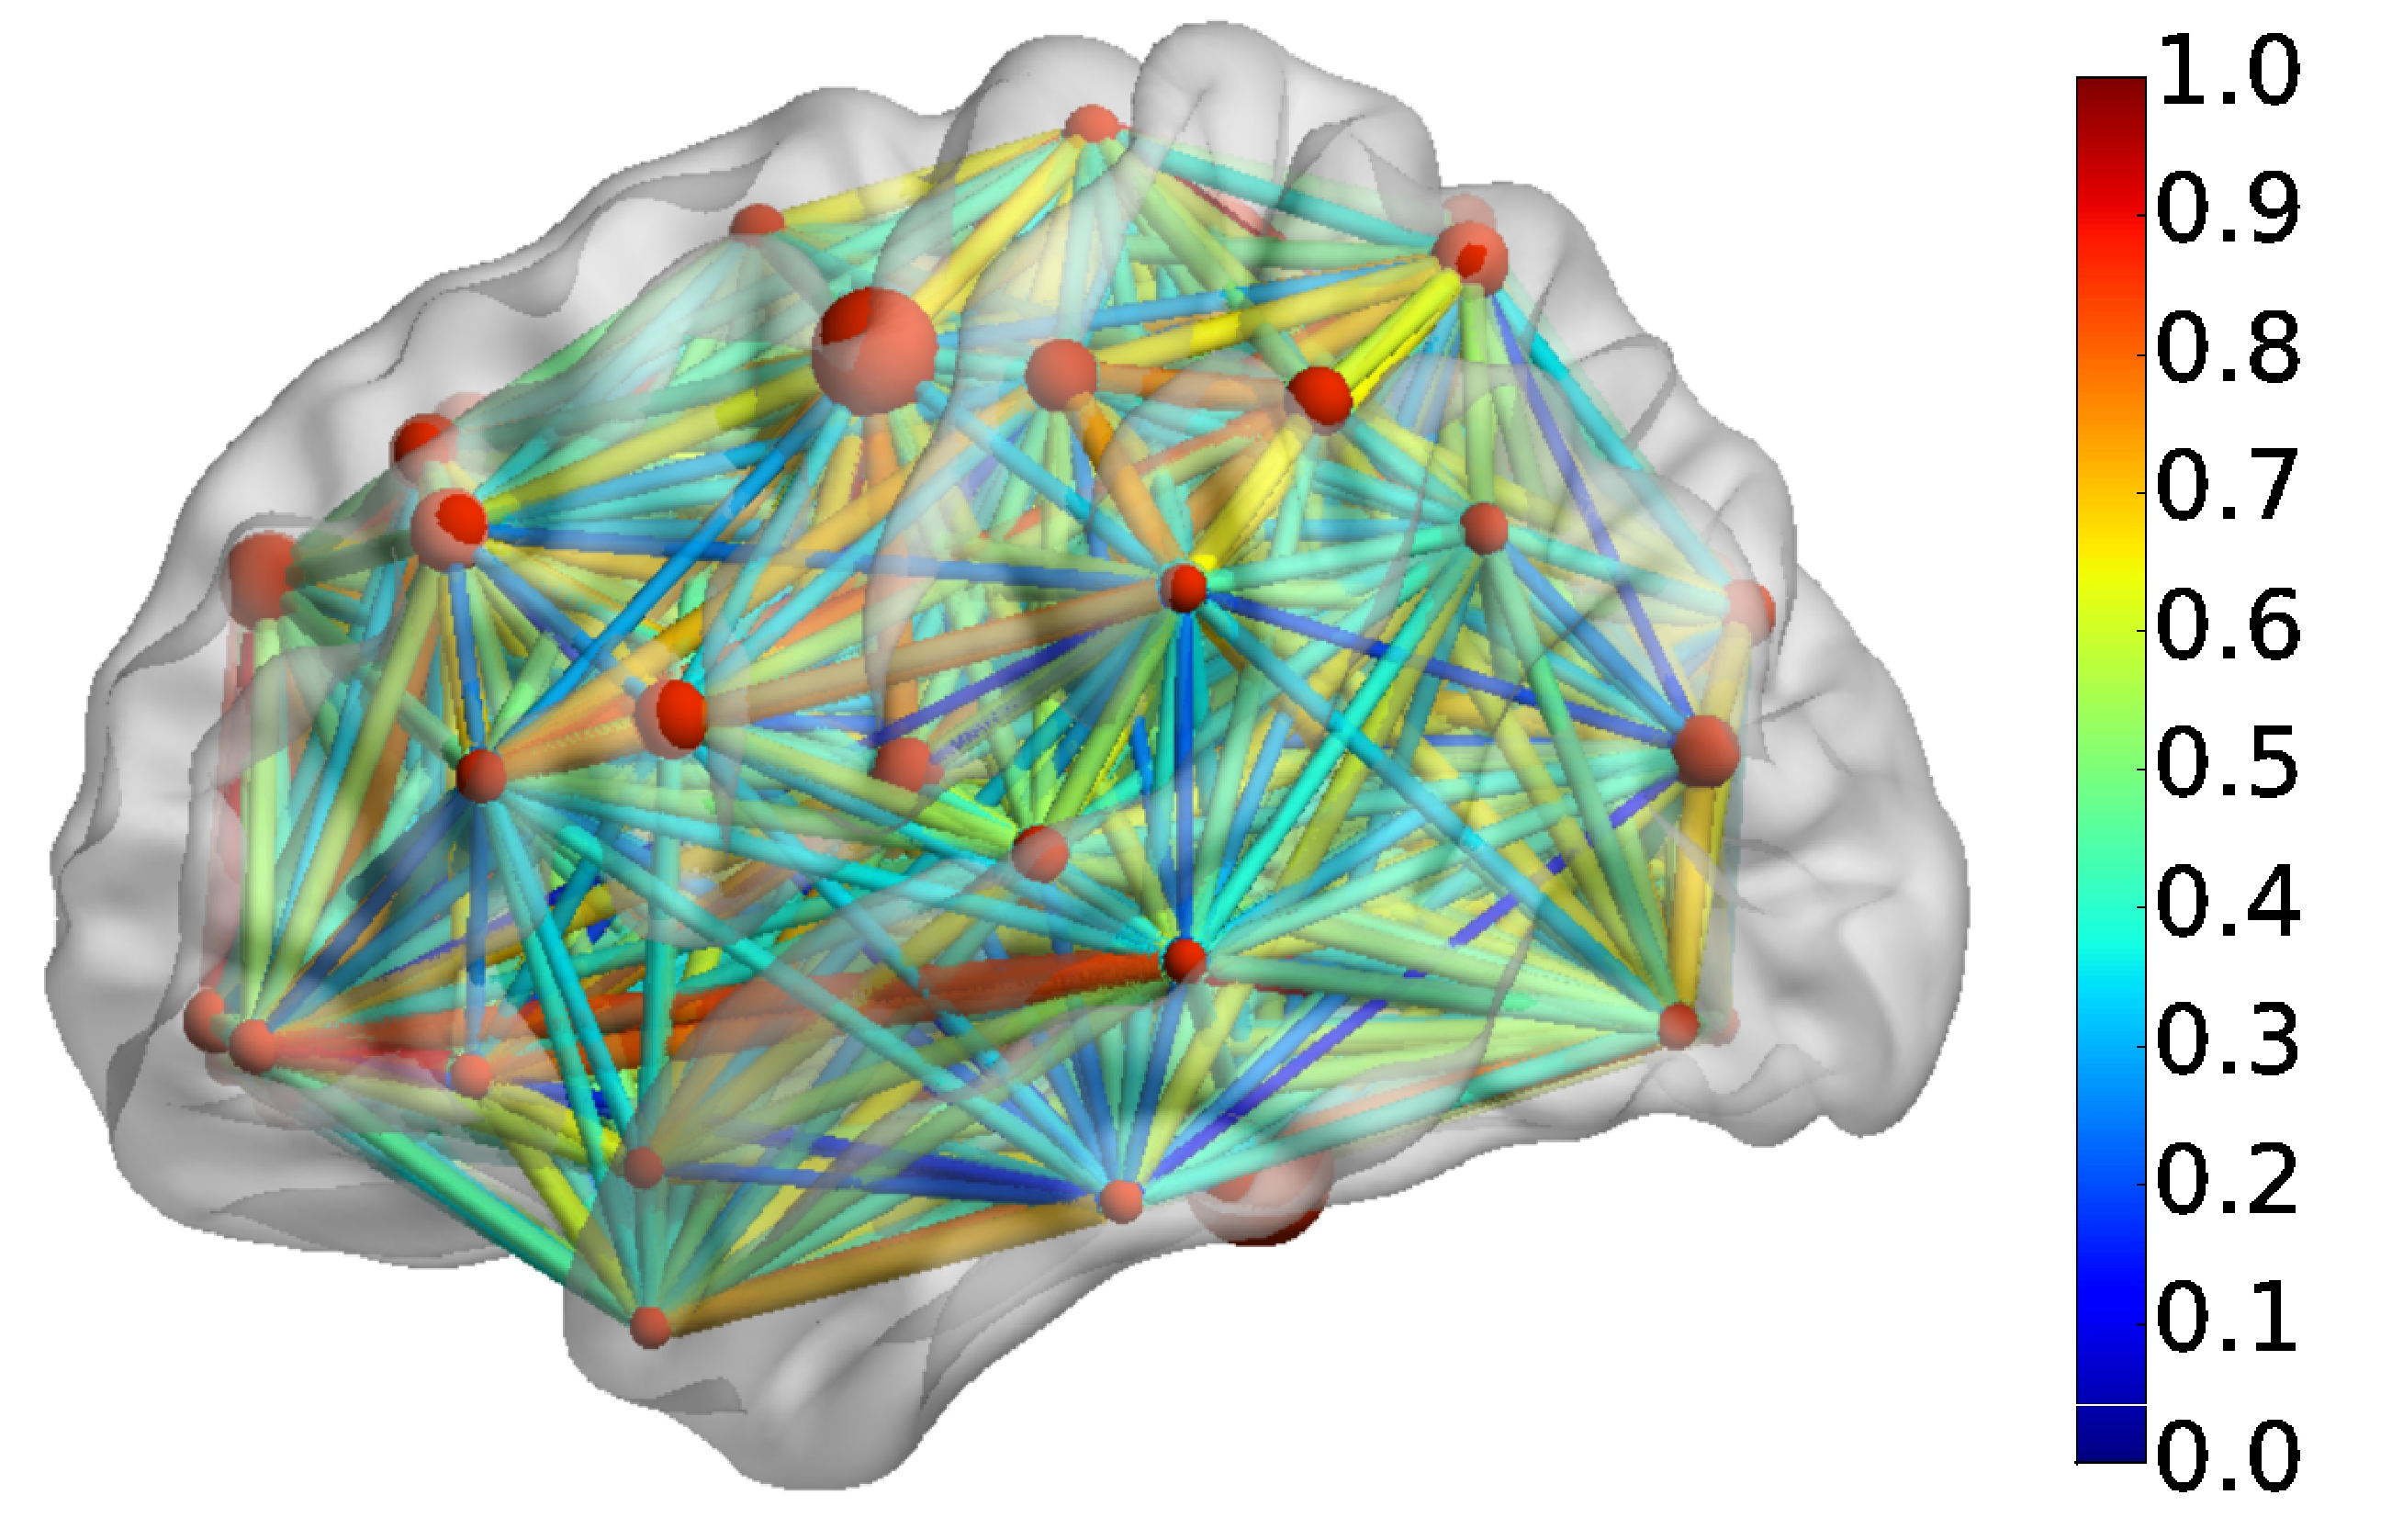
\includegraphics[width=0.49\textwidth]{Figures/FCM_brain.eps} 
	 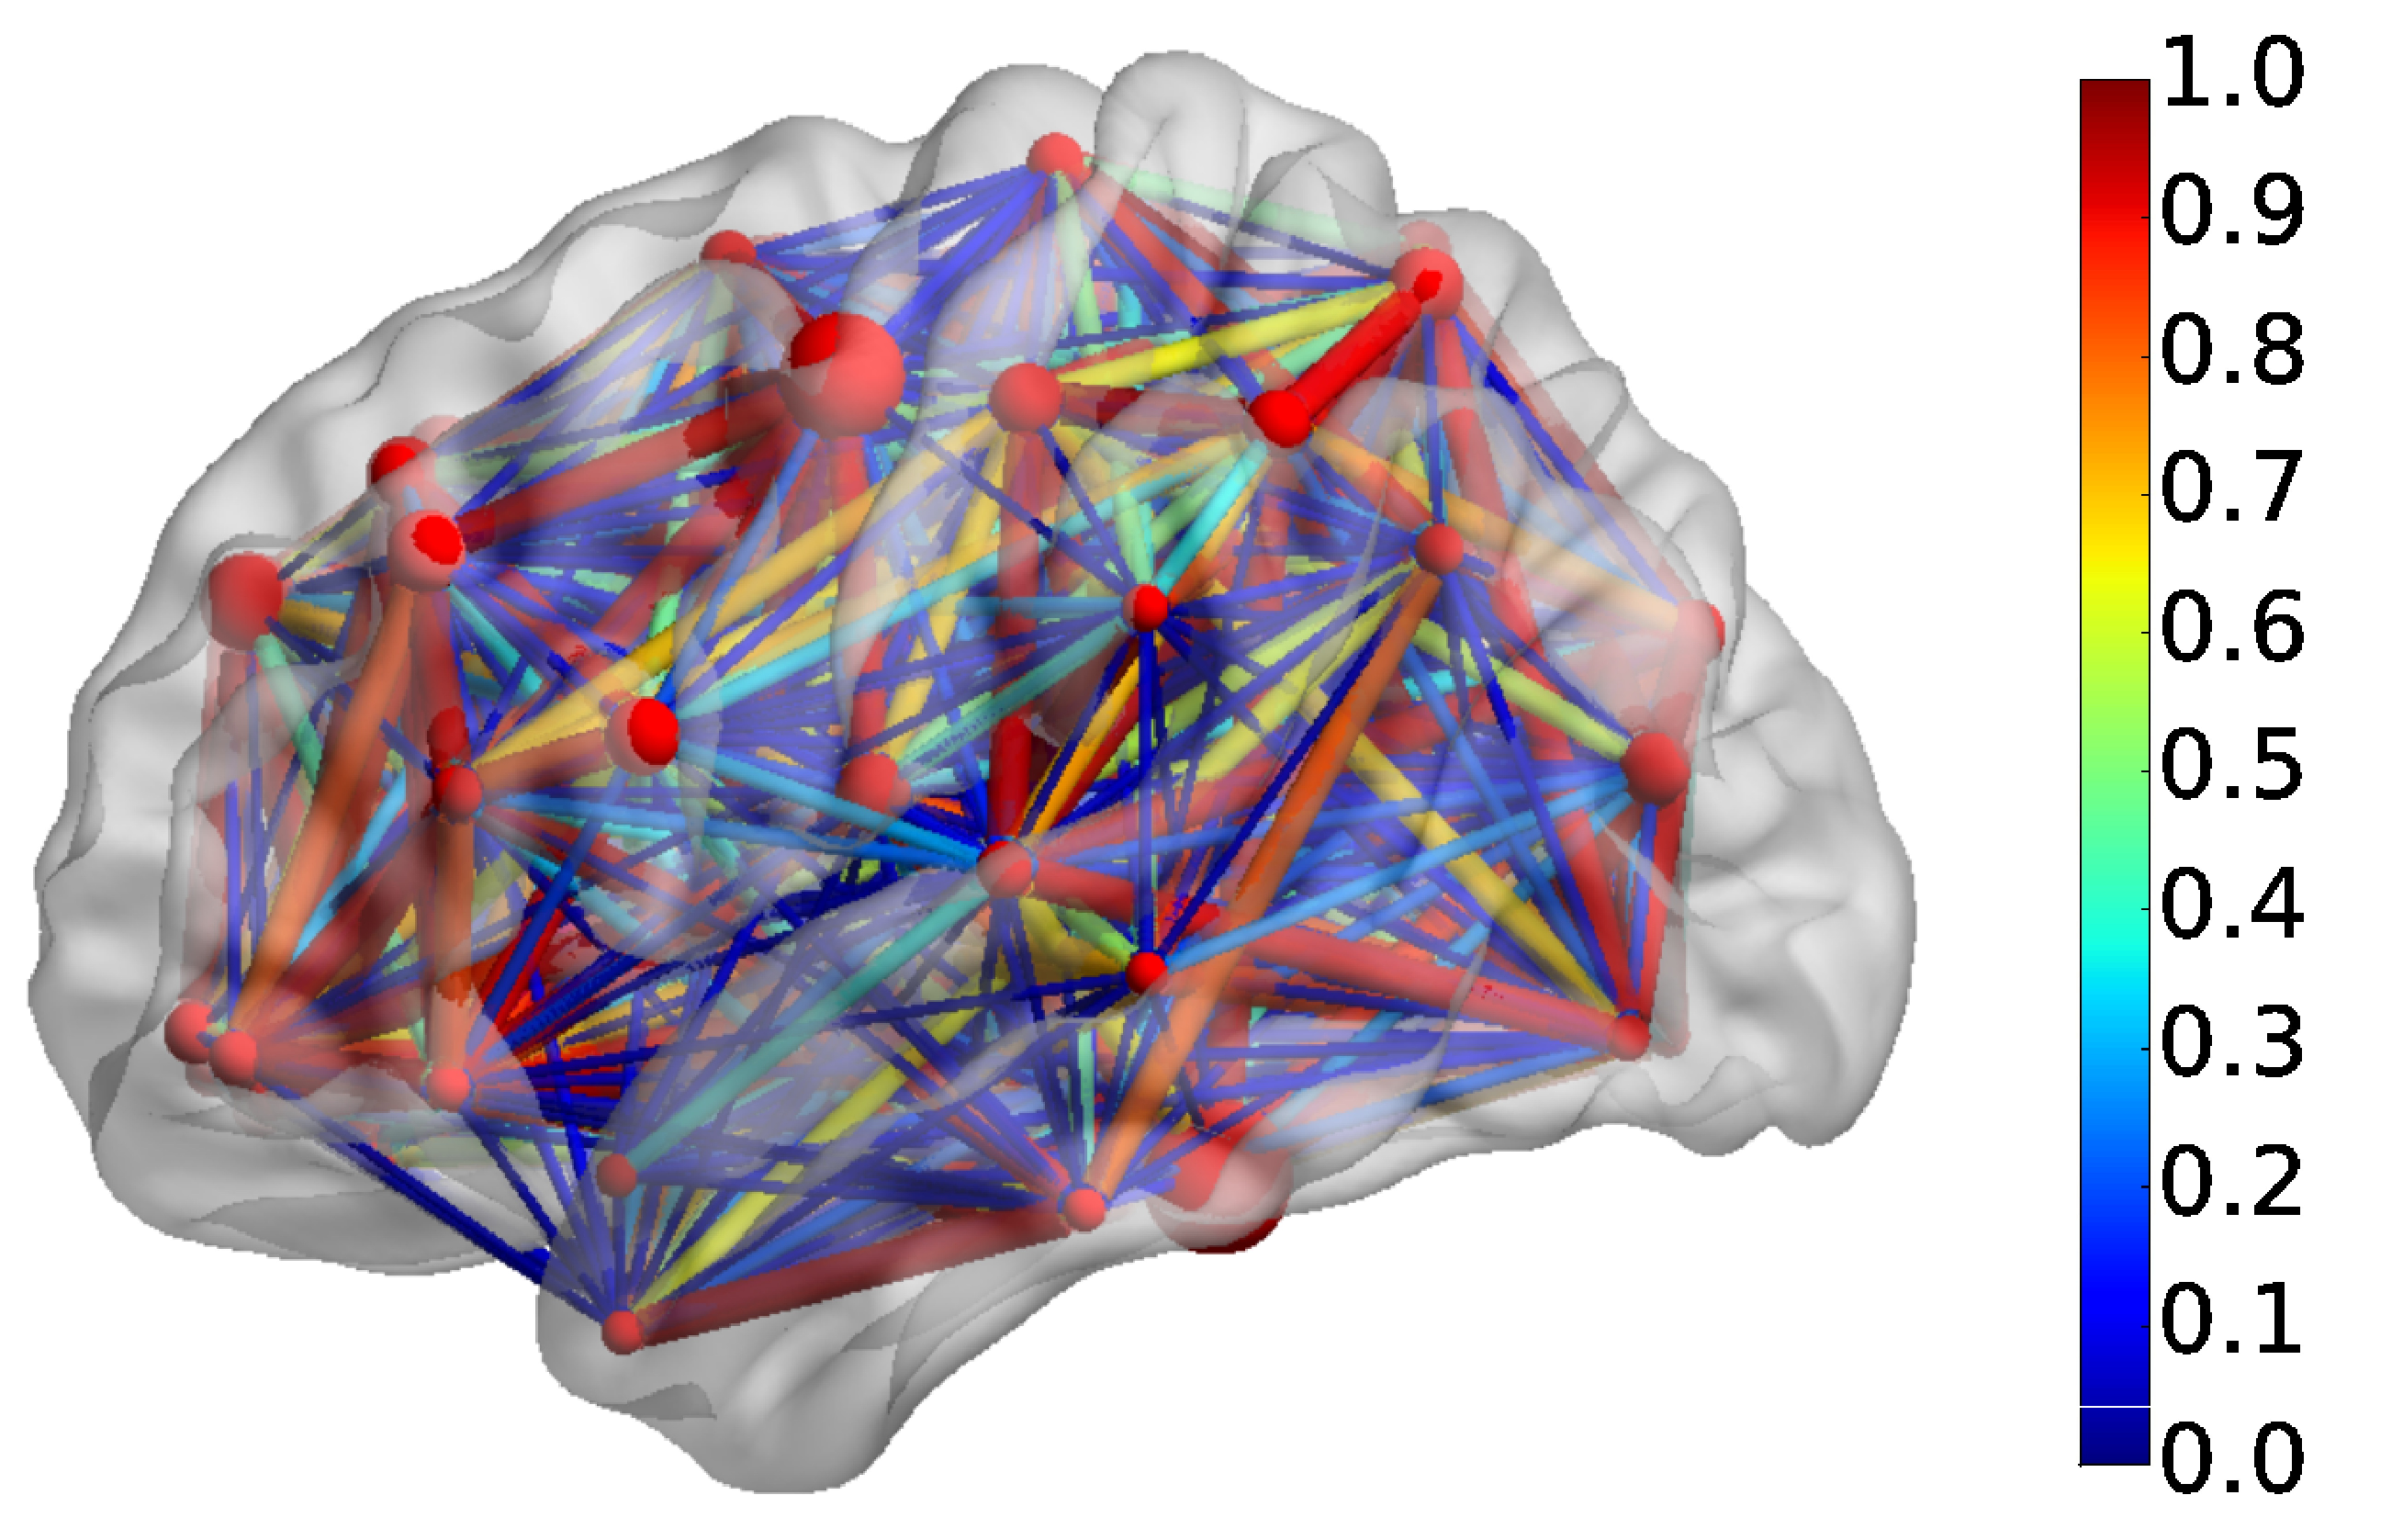
\includegraphics[width=0.49\textwidth]{Figures/ACM_brain.eps} 

\caption{3D sagittal visualization of empirical FC (left) and AC  maps (right) on the human cortex with the \textsc{BrainNet Viewer} \citep{XYZ13}. The colorbars are the same as explained in Figure \ref{fig:Empirical FCM and ACM}.  }
\label{fig:Empirical FCM and ACM in Cortex}
\end{figure}

Figure \ref{fig:Empirical FCM and ACM} represents empirically captured FC and AC matrices. All correlation coefficients in FC map appear in the range [0,1] as well as all probability values in AC map. Both matrices are symmetric. A correlation value close to 1 in FC matrix indicates that the quantified functional activities of corresponding nodes highly resemble each other (see sub-diagonals in Figure \ref{fig:Empirical FCM and ACM}, left). A probability value close to 1 in AC matrix demonstrates that corresponding nodes are most likely connected by fiber tracks in the white matter. Although some node pairs are not anatomically coupled at all in AC map (cold colors), they could be functionally coupled in FC map (hot colors). This is especially true for the corresponding regions in the different hemispheres.    

FC and AC matrices presented in Figure \ref{fig:Empirical FCM and ACM} are embedded in human cortex in Figure \ref{fig:Empirical FCM and ACM in Cortex} \citep{XYZ13}. The AAL regions are presented by red colored nodes with varying size dependent of \textit{nodal degree}. The \textit{edges} have different thickness and color distribution according to correlation coefficients and probability values with respect to FC and AC maps. The nerve fibers between nodes exist either with high (hot colors) or low (cold colors) probability (Figure \ref{fig:Empirical FCM and ACM in Cortex}, right). However, the functional correlations (Figure \ref{fig:Empirical FCM and ACM in Cortex}, left) tend to have an intermediate value (green colors). The distribution of anatomical and functional connections are clearly distinguishable in human brain.   



\subsection*{The Brain Graph and Erd\H{o}s-R\'{e}nyi-Type Random Graph}

\paragraph{The Brain Graph}

The brain graphs are generated through binarizing the empirical AC map via thresholding. We define a threshold value for the connection probability $p$ of node pairs. Then, the values greater and equal to $p$ are assigned the value 1, while others are set to 0. The resulting binary matrix is the basis of brain graph construction, and it is commonly known as \textit{adjacency matrix}. The \textsc{NetworkX} software package in \textsc{PYTHON} is used to built graphs given adjacency matrices \citep{XYZNETW}. Neither the direction of anatomical connectivity between nodes, nor any other values apart from 0 and 1  are encoded in the adjacency matrices so that the resulting graphs are considered as \textit{undirected} and \textit{unweighted}. In other words, all existing edges are thought to be of uniform weight and nodes interact both ways along an edge connecting them.


\paragraph{Erd\H{o}s-R\'{e}nyi-Type Random Graph}

Given a total number of nodes $N$, Paul Erd\H{o}s and Alfr\'{e}d R\'{e}nyi produced an undirected graph $G(N,P)$, in which the presence of any edge between two nodes is assigned a probability $P$. 
The average total number of edges $L$ in an  Erd\H{o}s-R\'{e}nyi-type random graph is $\binom {N} {2}P$, with a binomial distribution for the number of edges per node, known as the \textit{degree} of a node \citep{XYZERD}. 

New randomization techniques arise through modifying the Erd\H{o}s-R\'{e}nyi method, e.g. given $N$ and $L$, a graph can be picked uniformly random out of the set of all potential graphs having $N$ nodes and $L$ edges, which means the same \textit{network density} $\kappa$. The probability for a graph to be picked among all the others is $\frac{L}{\binom {N}{2}}$. (One can study the various aspects of $G(N,P)$ even more detailed \citep{NEW10}). 

In this study, we denote brain graphs as $R_{BG}$ and Erd\H{o}s-R\'{e}nyi-type random graphs as $R_{ER}$ for simplicity.

\begin{figure}[htpb]\centering
	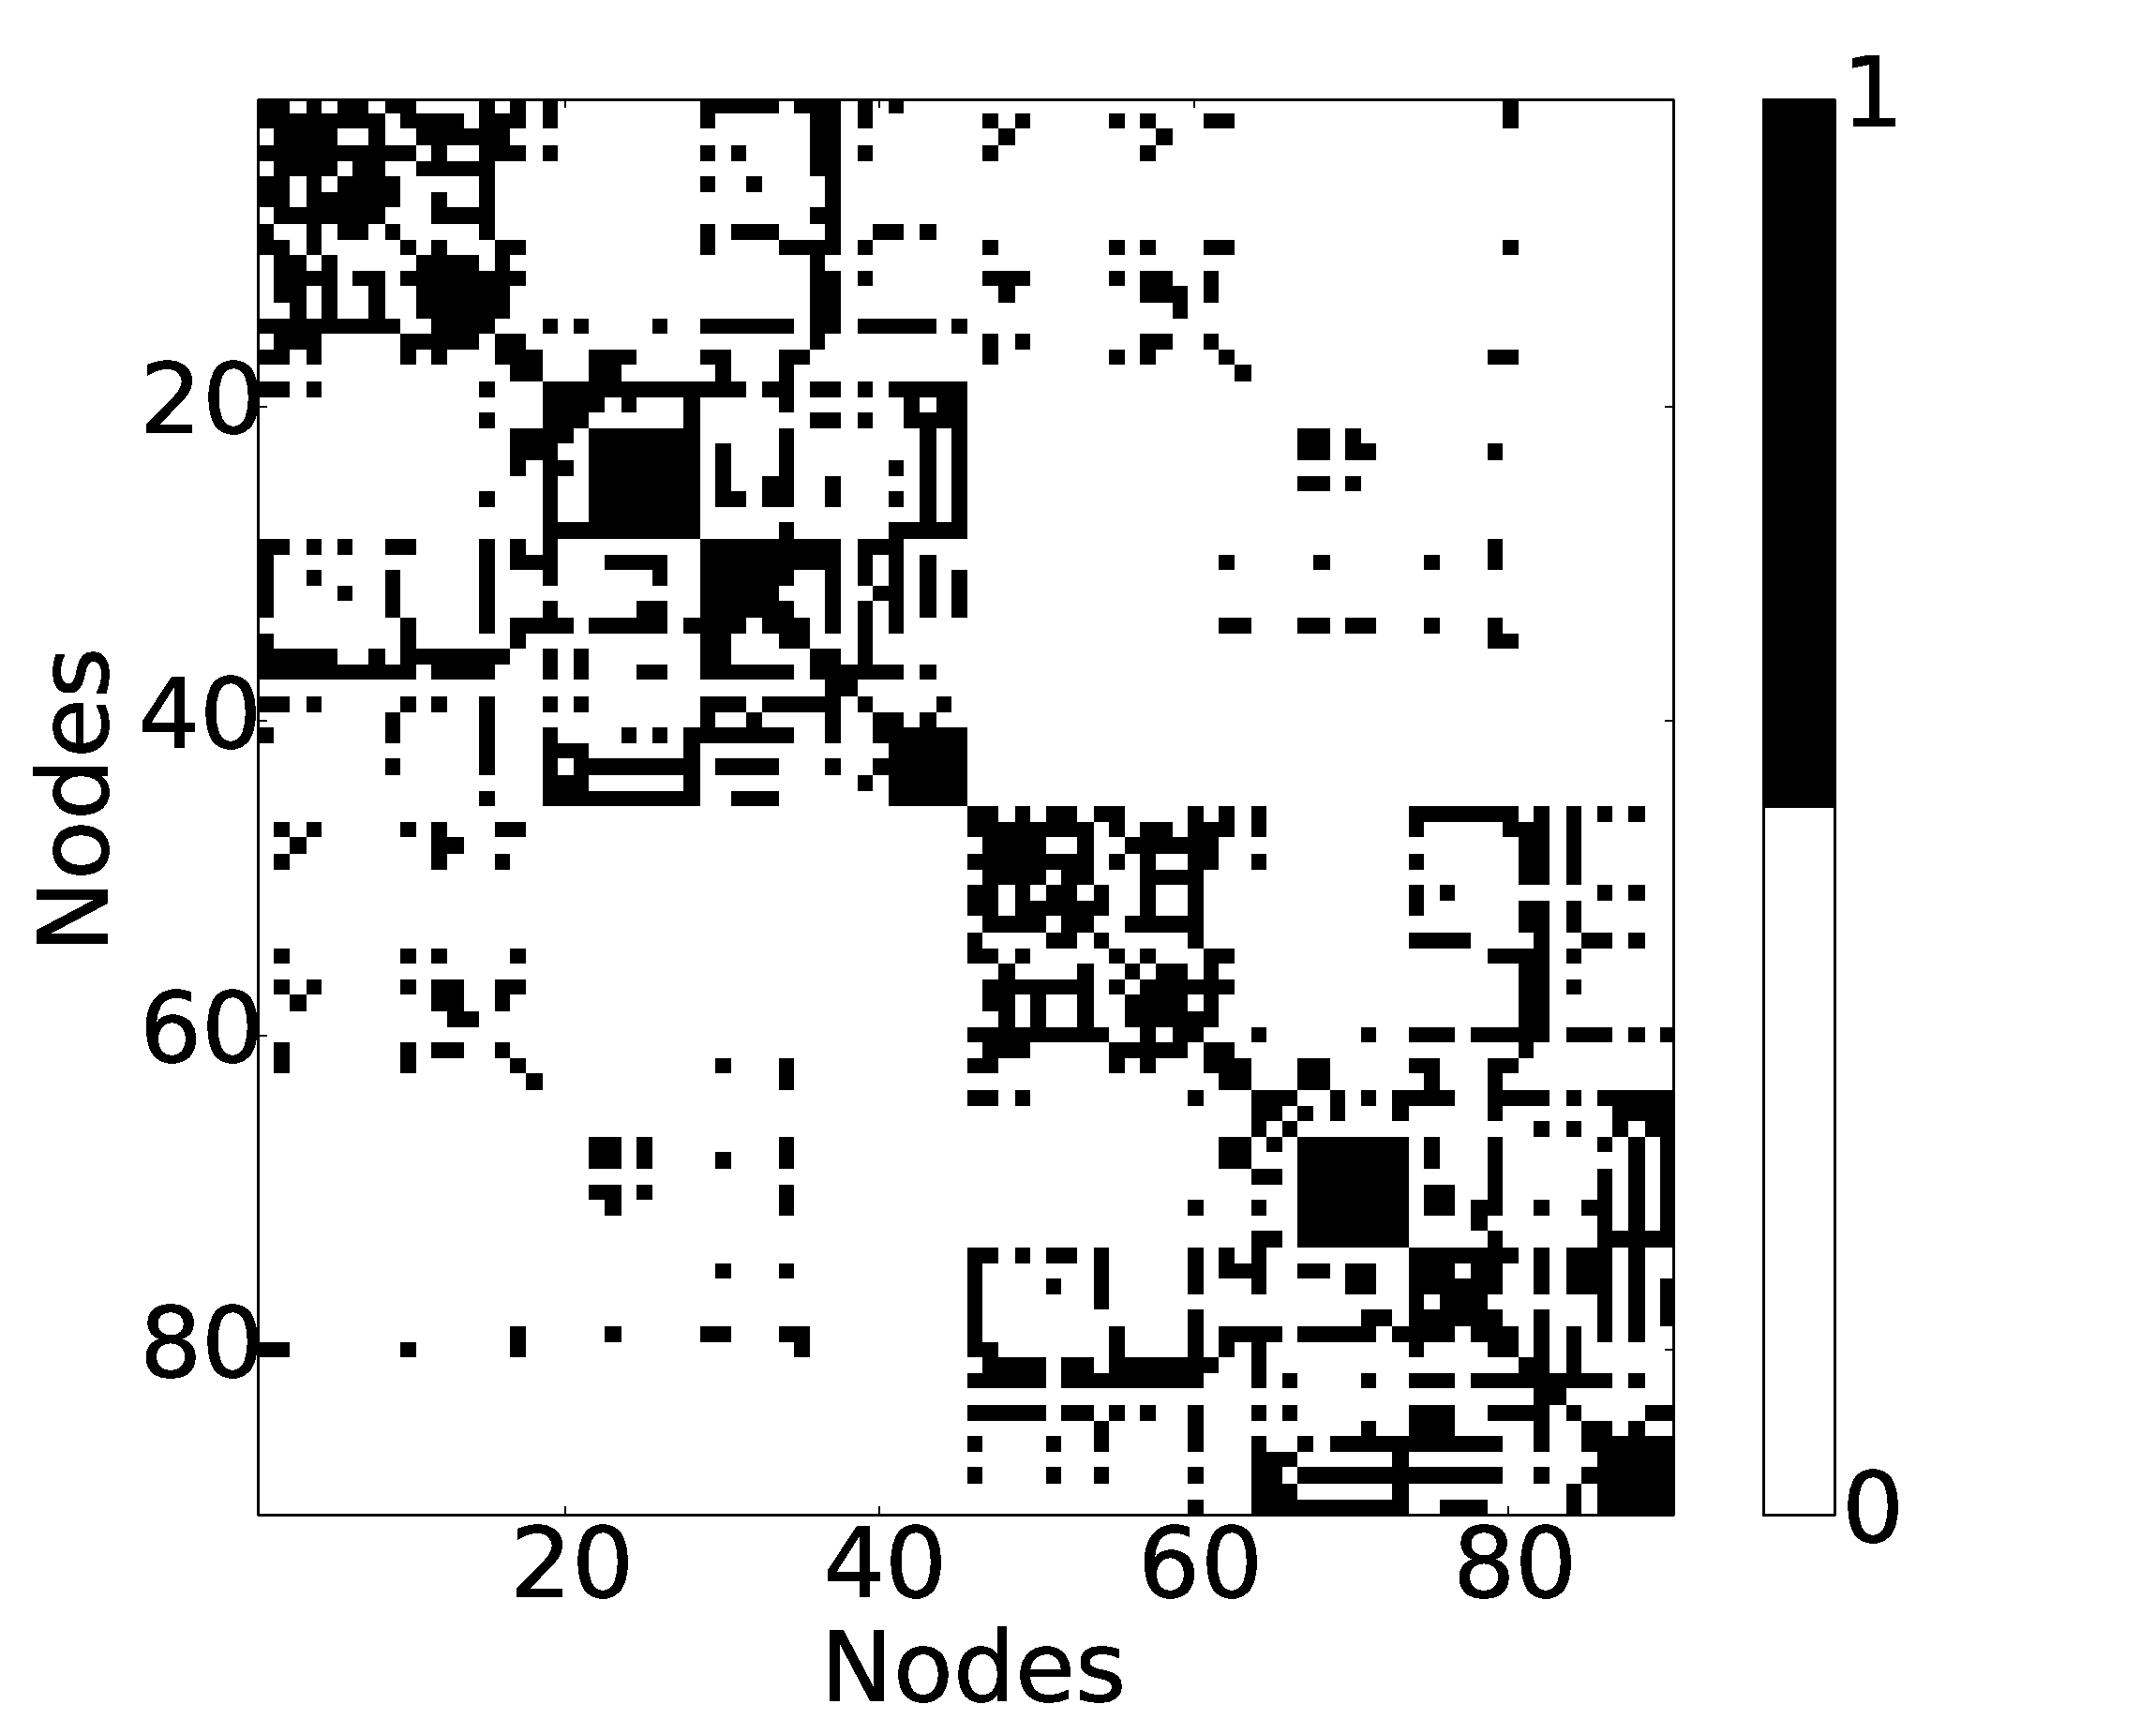
\includegraphics[width=0.49\textwidth]{Figures/Adj_ACM.eps}	 
	\includegraphics[width=0.49\textwidth]{Figures/Adj_ER.eps} 
	  
\caption{How to build adjacency matrices: The empirical AC map derived from DW-MRI technique is binarized at a connection probability value $p=0.54$ and its corresponding adjacency matrix is obtained (left). The black squares represent 1's indicating edges between nodes, whereas the white squares represent 0's implying no edge. The empirically derived adjacency matrix is manipulated via Erd\H{o}s-R\'{e}nyi randomization tool (right).}

\label{fig:Binarizing via Thresholding}
\end{figure}

Figure \ref{fig:Binarizing via Thresholding} illustrates the exemplary construction of adjacency matrices based on empirical connectivity map (left) as well as Erd\H{o}s-R\'{e}nyi method (right). Nodes are apparently densely connected intra-hemispherically (left), this pattern is coherent to the AC map seen in Figure \ref{fig:Empirical FCM and ACM} (right). However, there is no specific connection pattern as a result of randomization (right). The $\kappa$-value is preserved in the randomized matrix, but network topology differs. (See Appendix for a deeper understanding of network characteristics of $R_{BG}$ and $R_{ER}$.)   



\subsection*{FitzHugh-Nagumo Model for Neuronal Activity Simulations}

The theoretical model of choice for the neuronal activity is the FitzHugh-Nagumo (FHN) system phenomenologically describing physiological states of nerve membrane potential \citep{FIT61, NAG62}. The FHN model will be used to represent the neuronal time-series of a nerve cell population, in other words, an AAL node in this study. 

\paragraph{Local Dynamics}
Local dynamics described by FHN model has an activator variable $x$ and an inhibitor variable $y$. Their time evolution is represented with the same implementation as in \cite{GHO08, GHO08a} in the following nonlinear differential equations:

\begin{subequations}
\begin{align}\dot{x} = \tau \left( y + \gamma x - \frac{x^3}{3} \right)  \label{eqn: frobenius 1}\\  \dot{y} = -\frac{1}{\tau} (x - \alpha + b y - I ) , \label{eqn: frobenius 2}   \end{align} 
\end{subequations}

where time scale separation $\tau$ denotes the time constant accelerating $x$ and decelerating $y$, $I$ is the external stimulus parameter and $\gamma$, $\alpha$, $b$ are system parameters. $x$ and $y$ are considered to be counteracting variables capturing alterations of the membrane potential of a neuronal population of around $10^9$ cells. The parameters in the FHN model are tuned so that solutions render a damped oscillatory behavior for each node locally;  $\alpha = 0.85$, $b=0.2$, $\gamma=1.0$, $\tau=1.25$ and $I=0$ \citep{VUK13}. The fixed point of the system is a \textit{stable focus}.

\paragraph{Network Dynamics}

The FHN model to be simulated as the neuronal activity in the complete brain graph or random network is denoted with the following notation \citep{GHO08, VUK13},  
 
\begin{subequations}
 \begin{align}\dot{x_i} = \tau \left( y_i + \gamma x_i - \frac{x_i^3}{3} \right) -c \sum_{j=1}^N a_{ij}x_j(t - \Delta t_{ij}) +Dn_x \label{eqn: frobenius 17}\\  \dot{y_i} = -\frac{1}{\tau} (x_i - \alpha + b y_i - I ) +Dn_y \label{eqn: frobenius 18}  , \end{align} 
\end{subequations}

where indexes $i$ and $j$ represent any node among $N=90$ AAL regions, $c$ is the coupling strength, which scales the mutual time-delayed interactions, $a_{ij}$ is the corresponding element of the adjacency matrix obtained at a specific $p$-value, $n_x$, $n_y$ represent Gaussian white noise sources with zero mean and unity variance and $D$ is the noise strength.
If nodes are connected in a given network, then $a_{ij}=1$, otherwise $a_{ij}=0$. $\Delta t_{ij}$ is the time-delay factor arising from finite signal propagation velocity $v$ among nodes. $\Delta t_{ij}$ is calculated as $\Delta t_{ij}=\frac{d_{ij}}{\nu}$ \citep{GHO08, GHO08a, DEC09}, where $d_{ij}$ is the distance matrix for the approximated fiber lengths between AAL regions from which AC map is constructed \citep{ITU08} (Figure \ref{fig:d_ij}). The strength of noise is $D=0.05$. The noise variable drives subthreshold oscillations, the system does not settle down to the fixed point, indicating loss of stability.


\begin{figure}[htpb]\centering
	 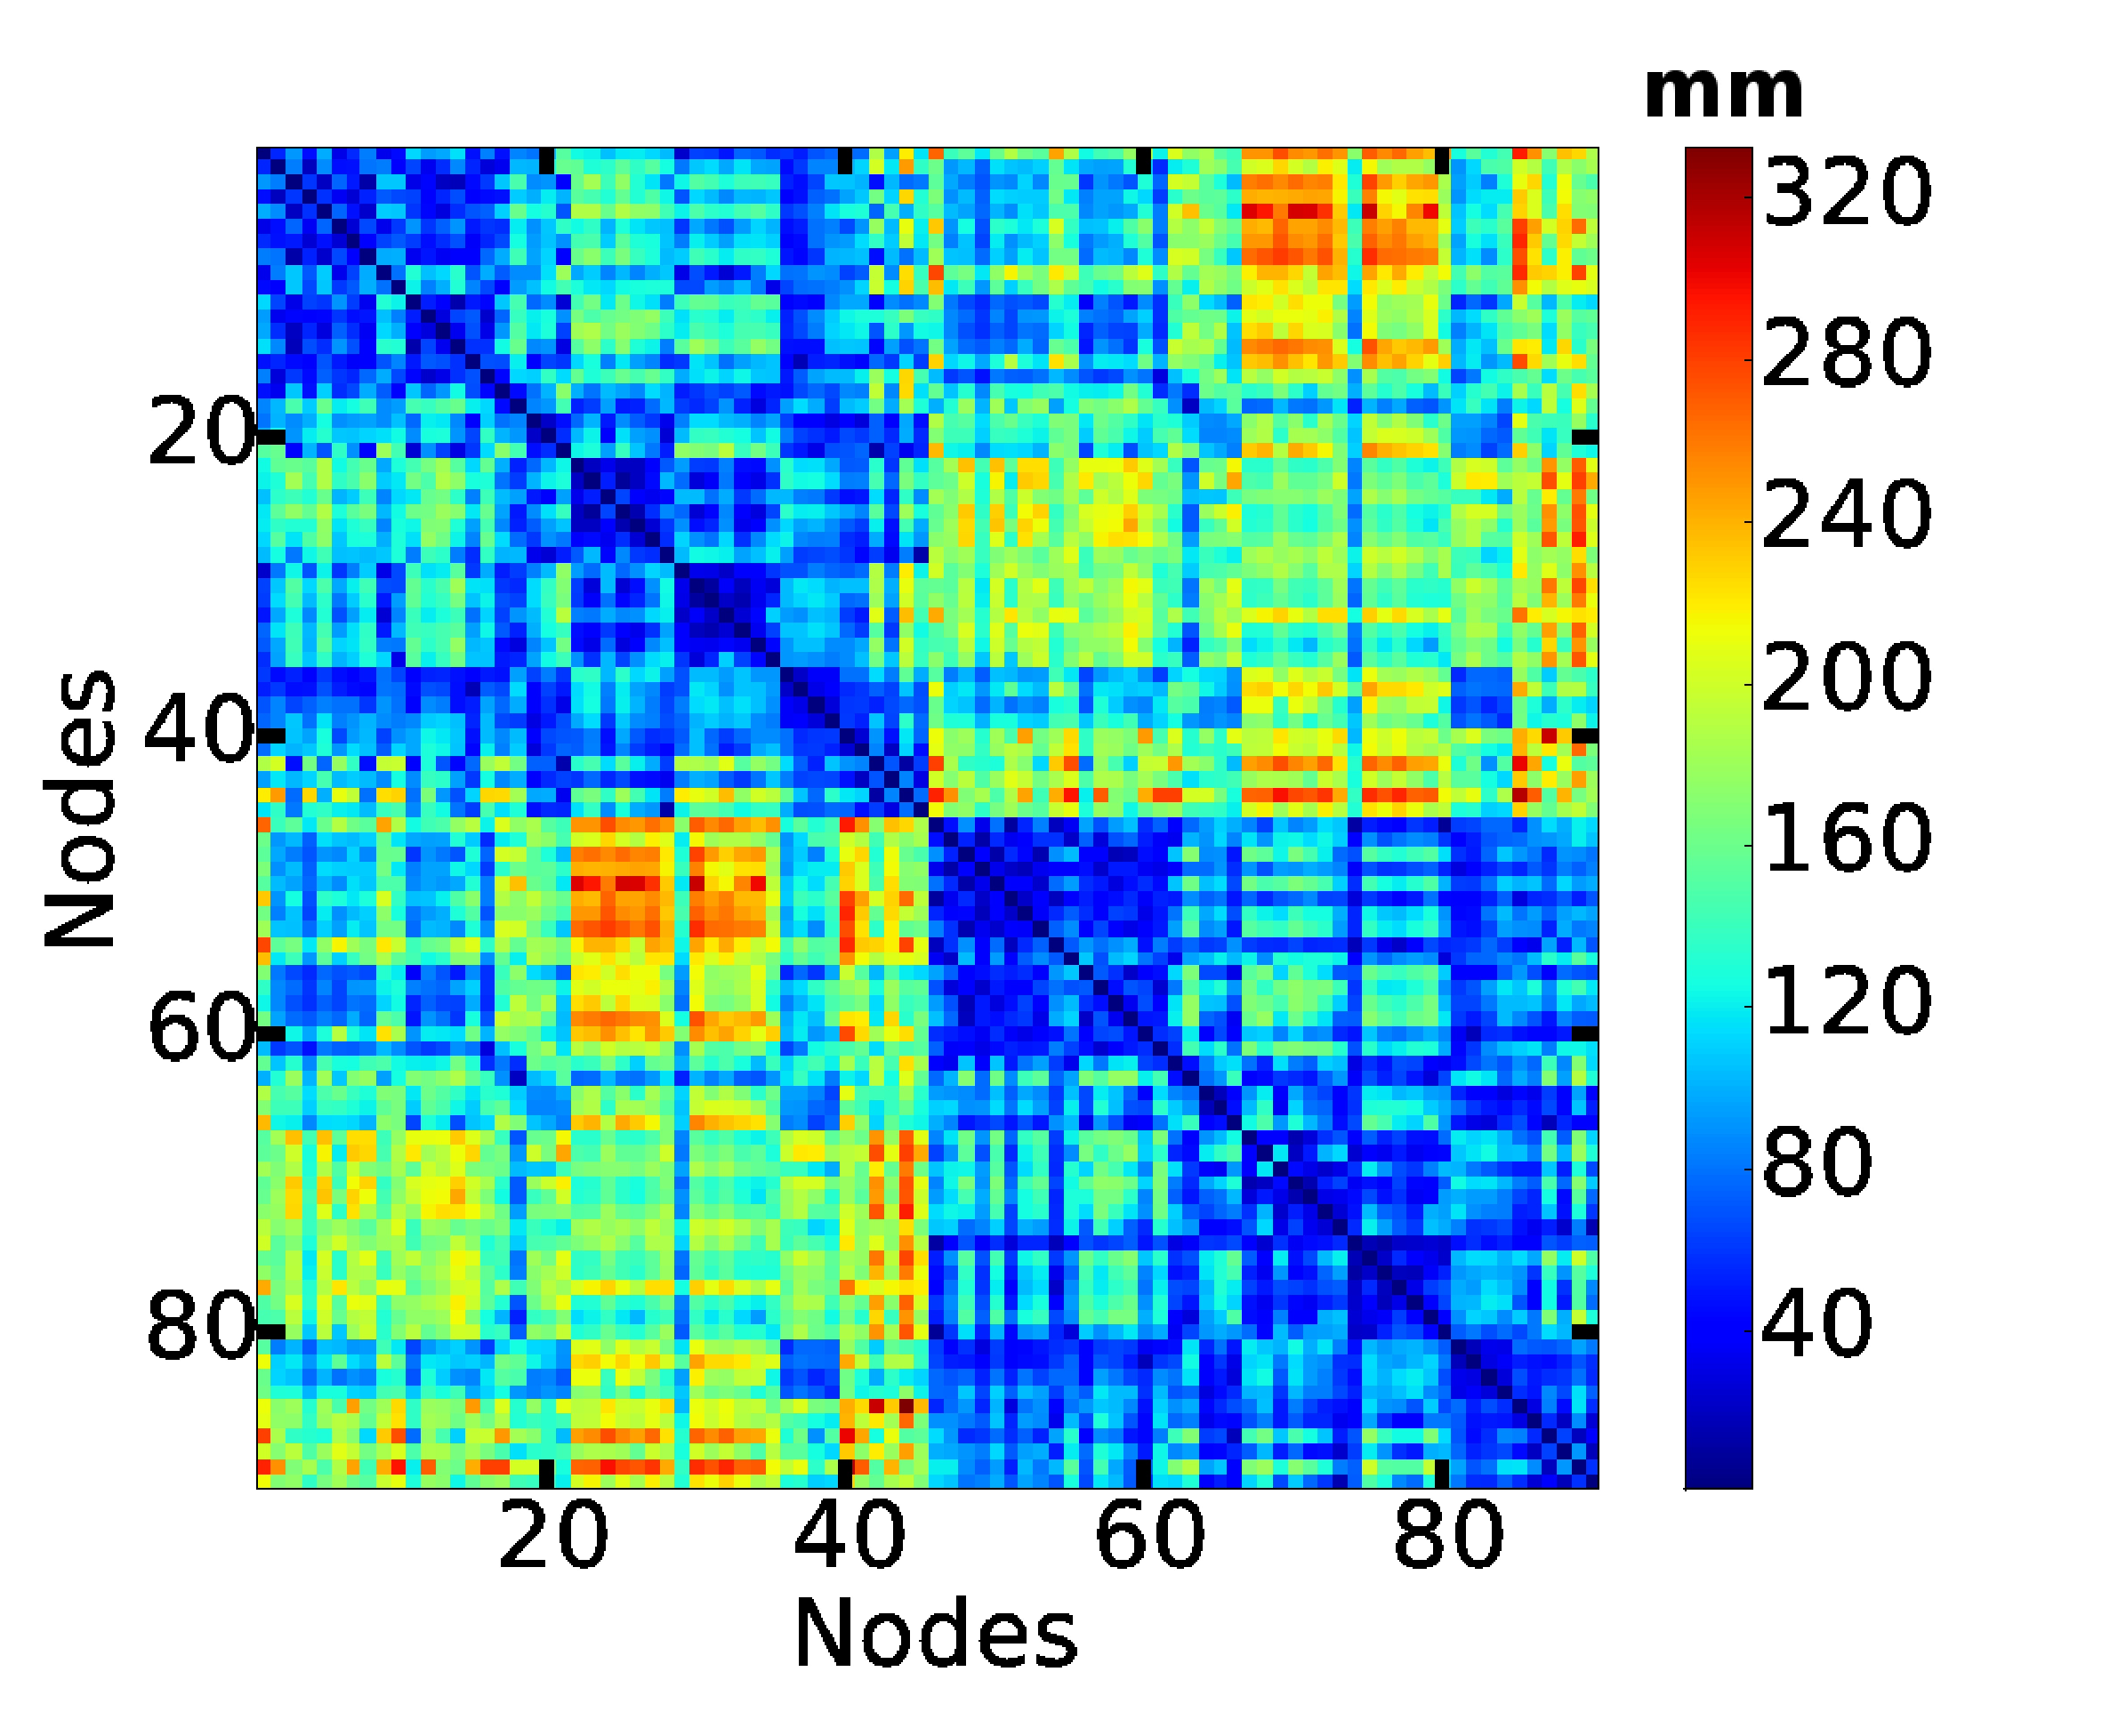
\includegraphics[width=0.49\textwidth]{Figures/distance_ACM_pyt.eps} 
	
\caption{Distance matrix $d_{ij}$(mm) symbolizing the approximate fiber length between node pairs}
\label{fig:d_ij}
\end{figure}


The time delay coupled set of ordinary differential equations is solved numerically with \textsc{PYTHON}-module \textsc{PYDELAY}-algorithm (\textit{http://pydelay.sourceforge.net}) based on Bogacki-Shampine method \citep{BOG89, FLU09a}. The FHN model is designed to reflect the neuronal activity as a simulated time-series. $N=90$ nodes in any given network are be simulated with the complete FHN timse-ries notation for 7.5 minutes.  

\subsection*{Balloon-Windkessel Model for BOLD Activity Simulation} 
The modeled neuronal activity is used to infer the BOLD signal observed in the fMRI data via the Balloon-Windkessel hemodynamic process, which mediates between a non-linear time-series and all the measured BOLD response \citep{FRI00}. In short, the Balloon-Windkessel model picks an input signal in the form of neuronal time-series and generates the hemodynamic oscillations analogous to the BOLD signal, which is modeled as a function of changes in cerebral blood flow, cerebral blood volume and cerebral metabolic rate of oxygen consumption. 

The main input of the Baloon-Windkessel model is a neuronal signal in the form of either a spiking rate or a local field potential \citep{SET12}. The neuronal signal in this project will be the normalized FHN time-series of an activator variable, which describes the excitatory membrane potential dynamics of a neuronal population. The study of \cite{FRI00} shows that it is possible to capture ultra-slow frequency oscillations ($<0.1$ Hz) in the hemodynamic process, given a higher frequency neuronal input for event related responses. Here, the same model will be tested for the resting-state activity to find out whether it is possible to extract BOLD activity from FHN-modeled $N=90$ AAL brain nodes.


\subsection*{Comparing Simulated and Empirical Correlation Matrices}       

One of the research proposals of this paper is to investigate whether the functional connectivity (FC) in human brain at resting-state can be captured through its anatomical connectivity (AC). To answer this question, the brain graphs obtained from AC map are simulated with BOLD activity and then the results are compared statistically to the FC map.

The correlation of simulated BOLD activity between any node pairs $i,j$ is quantified by Pearson's correlation coefficient $\rho_{i,j}$, 

\begin{equation}
\rho_{i,j} = \dfrac{\big \langle u_i(t) u_{j}(t) \big \rangle - \big \langle u_{i}(t) \big \rangle  \big \langle u_{j}(t) \big \rangle}{ \sigma (u_i(t)) \sigma (u_j(t))}
\end{equation}

where $u_i(t)$ denotes the BOLD time-series of the corresponding node $i$,  $\sigma$ stands for standard deviation and $\big \langle \cdot \big \rangle$ represents the temporal average. 

All $\rho_{i,j}$ values among any possible pairwise combination of $N=90$ nodes are then used to built a $90\times 90$  matrix, which is referred to as simulated functional connectivity (FC$_s$). 

In order to compare the modeling approach to the empirical result, the FC$_s$ and the empirical FC map (FC$_e$) derived from fMRI-BOLD measurements are compared statistically with Pearson's correlation coefficient, the same linear pairwise correlation method again. All correlation values $\rho_{e,s}$ between empirical $e$ and simulated $s$ data matrices will be placed in the parameter space $(p,c)$. 

\subsection*{Comparing Brain Graphs to Random Graphs}
$R_{BG}$ and $R_{ER}$ are compared not only in terms of their network measures but also their modeled temporal dynamics, which is obtained with FHN network model and BOLD activity simulations. The Pearson correlation coefficients $\rho$ between any pairwise combinations of $N=90$ nodes are calculated for their modeled time-series in each network. These correlation coefficients are then distributed in histograms at $(p,c)$-values. In order to quantify the analogy of modeled temporal activity between $R_{BG}$ and $R_{ER}$, we calculate Bhattacharya coefficients, a widely used statistical approach to measure the correlation between statistical samples, i.e. histograms \citep{XYZ43}.

Let us denote the $\rho_{i,j}$ histogram distributions of simulated temporal activity of $R_{BG}$ with $H_b$ and that of $R_{ER}$ with $H_r$, the Bhattacharya coefficient $d(H_b, H_r)$ is given by the following equation:

\begin{equation}
d(H_b, H_r) = \sqrt{1- \dfrac{1}{ \sqrt{\bar{H_r} \bar{H_b} N^2}} \sum_{i} \sqrt{H_r(i)H_b(i)} } ,
\end{equation}

where $\bar{H}$ denotes the mean of histogram \citep{XYZ43}. $d(H_b, H_r)$ is scaled between 0 and 1. A high $d(H_b, H_r)$ value indicates a low correlation between $H_b$ and $H_r$, whereas a low   $d(H_b, H_r)$ value expresses a high degree of similarity. 



\section*{Results \& Discussion}

\subsection*{Network Measures of Brain Graph vs Random Graph}

The topological properties of $R_{BG}$ and $R_{ER}$ are illustrated with some of the key network measures in Figure \ref{fig:network measures}. $\kappa$, \textit{average clustering coefficients} $C$, and  \textit{small-worldness} $S$ of each network are calculated and visualized in dependence of $p$-values (See Appendix). Figure \ref{fig:network measures} (left) shows that $\kappa$ of $R_{BG}$ is preserved in $R_{ER}$, as expected from the definition of Erd\H{o}s-R\'{e}nyi-type randomization. $\kappa$ decreases sigmoidally with increasing $p$. Figure \ref{fig:network measures} (middle) indicates that $R_{BG}$ has higher $C$-values compared to $R_{ER}$, meaning that nodes in $R_{BG}$ tend to cluster more. Therefore, the local information transfer is expected to be more efficient in $R_{BG}$. The networks are clearly distinguishable in terms of $S$-values as seen in Figure \ref{fig:network measures} (right). Random networks seem to be equally segregated and integrated in general, but the real networks behave differently. 



\begin{figure}[ht]\centering
	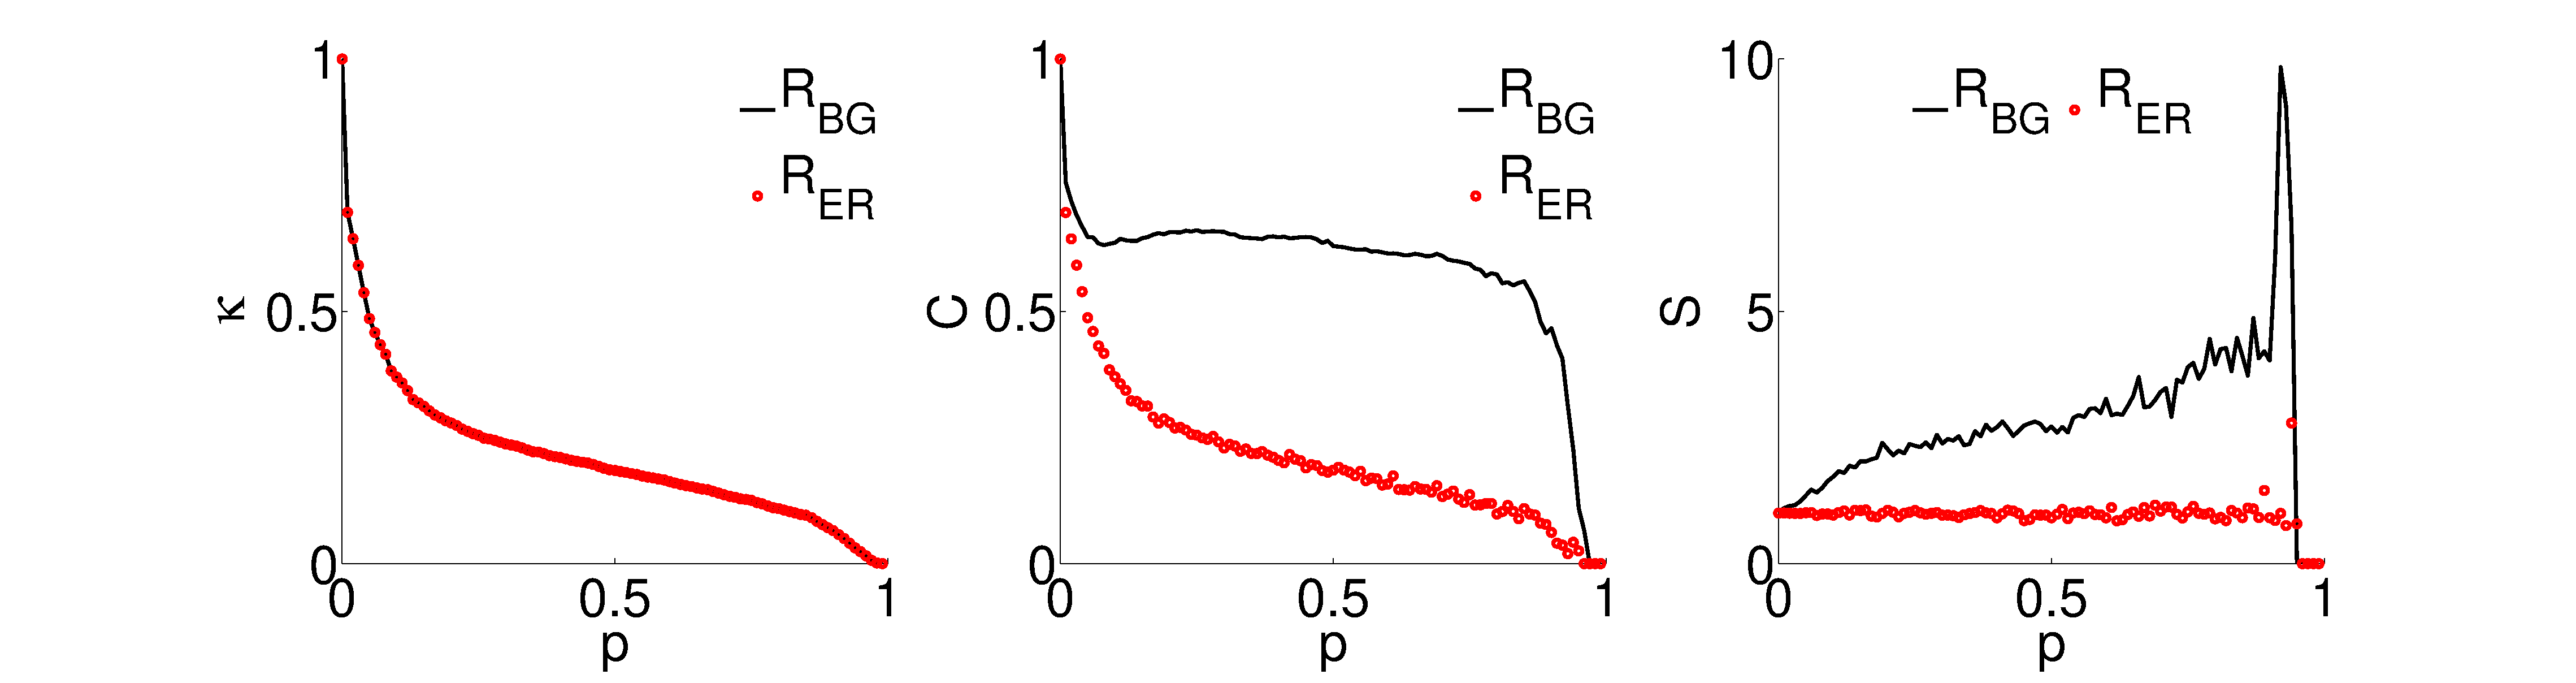
\includegraphics[width=\textwidth]{Figures/network_meas.eps}  
\caption{$\kappa$, $C$ and $S$ statistical network characteristics of $R_{BG}$ and $R_{ER}$. Black curves indicate $R_{BG}$ and red dots denote $R_{ER}$ network measures. }
\label{fig:network measures}
\end{figure}

\newpage
\subsection*{Modeled BOLD Activity on Anatomical Connectivity Map}

For each set of $(p,c)$, we built a simulated functional connectivity matrix FC$_s$ for the modeled BOLD signal. The FC$_s$ and empirically derived functional connectivity matrix FC$_e$ (Figure \ref{fig:Empirical FCM and ACM}, left) are compared quantitatively by Pearson's correlation coefficients $\rho_{e,s}$ in parameter space of $(p,c)$. The results are demonstrated in Figure \ref{fig:PA_p_c}.

% We investigated that it would be possible to capture functional activity at resting-state through the anatomical connectivity in human brain. 

\begin{figure}[ht]\centering

	\includegraphics[width=0.57\textwidth]{Figures/PA_ACM_BOLD_v_3.eps}  
\caption{Parameter analysis for the statistical comparison of FC$_s$ and FC$_e$ in $(p,c)$-space. The FC$_e$ is unique and refers to the FC map in Figure \ref{fig:Empirical FCM and ACM} (left). Several FC$_s$ matrices are obtained via modeling BOLD temporal dynamics on the AC map, which is shown in Figure \ref{fig:Empirical FCM and ACM} (right). The colorbar represents $\rho_{e,s}$ between empirical and simulated matrices. The results are exhibited for weekly coupled functional interactions with low $c$-values. $p$-values are considered to be between 0.18 and 0.82 by increment of 0.04. The signal propagation velocity $v$ is fixed as 3 m/s.}
\label{fig:PA_p_c}
\end{figure}

 In Figure \ref{fig:PA_p_c}, the statistical match between simulated and empirical BOLD activity correlations tend to be high at relatively low coupling strengths $c \leq 0.1$ and connection probability $0.18 <p<0.70$ as visualized by hot colors. In particular, it can be inferred that, the smaller scaled the neuronal activity oscillations are, the higher correlation between FC$_s$ and FC$_e$ is captured. Here, the range of $p$-values resulting in high agreement point out a network density $ 0.29 > \kappa > 0.14$. The magnitude of $\kappa$ is in agreement with the study of \cite{BUL11} regarding to a convincing network topology. It should be also mentioned, that the signal propagation velocity $v$ is fixed to 3 m/s, which corresponds to the lower boundary for a biophysically plausible signal velocity range \citep{GHO08}. 



\begin{figure}[htpb]\centering
	 \includegraphics[width=0.49\textwidth]{Figures/cor_BOLD_ACM_sim.eps} 
%   	 \includegraphics[width=0.49\textwidth]{Figures/cor_FCM_exp.eps} 

  \caption{A simulated functional connectivity matrix FC$_s$ captured from hot colored squares in Figure \ref{fig:PA_p_c} (right), corresponding to $\rho_{e,s} = 0.22$. Modeling parameters are $p=0.54$, $c=0.03$ and $v=3$. } 
    \label{fig:BOLD_e_s}
 	
\end{figure}  


The best analogy between FC$_s$ and FC$_e$ is captured at $c=0.03$ and $p=0.54$ with $\rho_{e,s}=0.22$ as seen in Figure \ref{fig:PA_p_c}. Figure \ref{fig:BOLD_e_s} illustrates the FC$_s$ matrix at these particular parameter values. Here, the colorbar denotes the pairwise Pearson's coefficients $\rho_{i,j}$ between the modeled BOLD time-series of all possible node pairs ${i,j}$. The FC$_e$ in Figure \ref{fig:Empirical FCM and ACM} (left) indicates 
well correlating measured BOLD signals of AAL pairs located inter- and intra-hemispherically, as seen  along the main diagonal and sub-diagonals. The FC$_s$ tends to capture these well correlations along the main diagonal, however, it almost fails to catch the ones on the sub-diagonals. Top left quadrants (nodes in left hemisphere $i,j=\{1,2,...,45\}$) and bottom right quadrants (nodes in right hemisphere $i,j=\{46,47,...,90\}$) in both matrices correlate with higher Pearson coefficients: $\rho_{e,s}(LL)=0.40$ and $\rho_{e,s}(RR)=0.52$. The FC$_s$ does not exhibit high correlating inter-hemispheric nodes as dominant as in FC$_e$. The longer distances between right and left hemispheric nodes might be the reason, why our model cannot successfully reproduce the inter-hemispheric correlations (see Figure \ref{fig:d_ij}). 
    

\begin{figure}[htpb] \centering
	 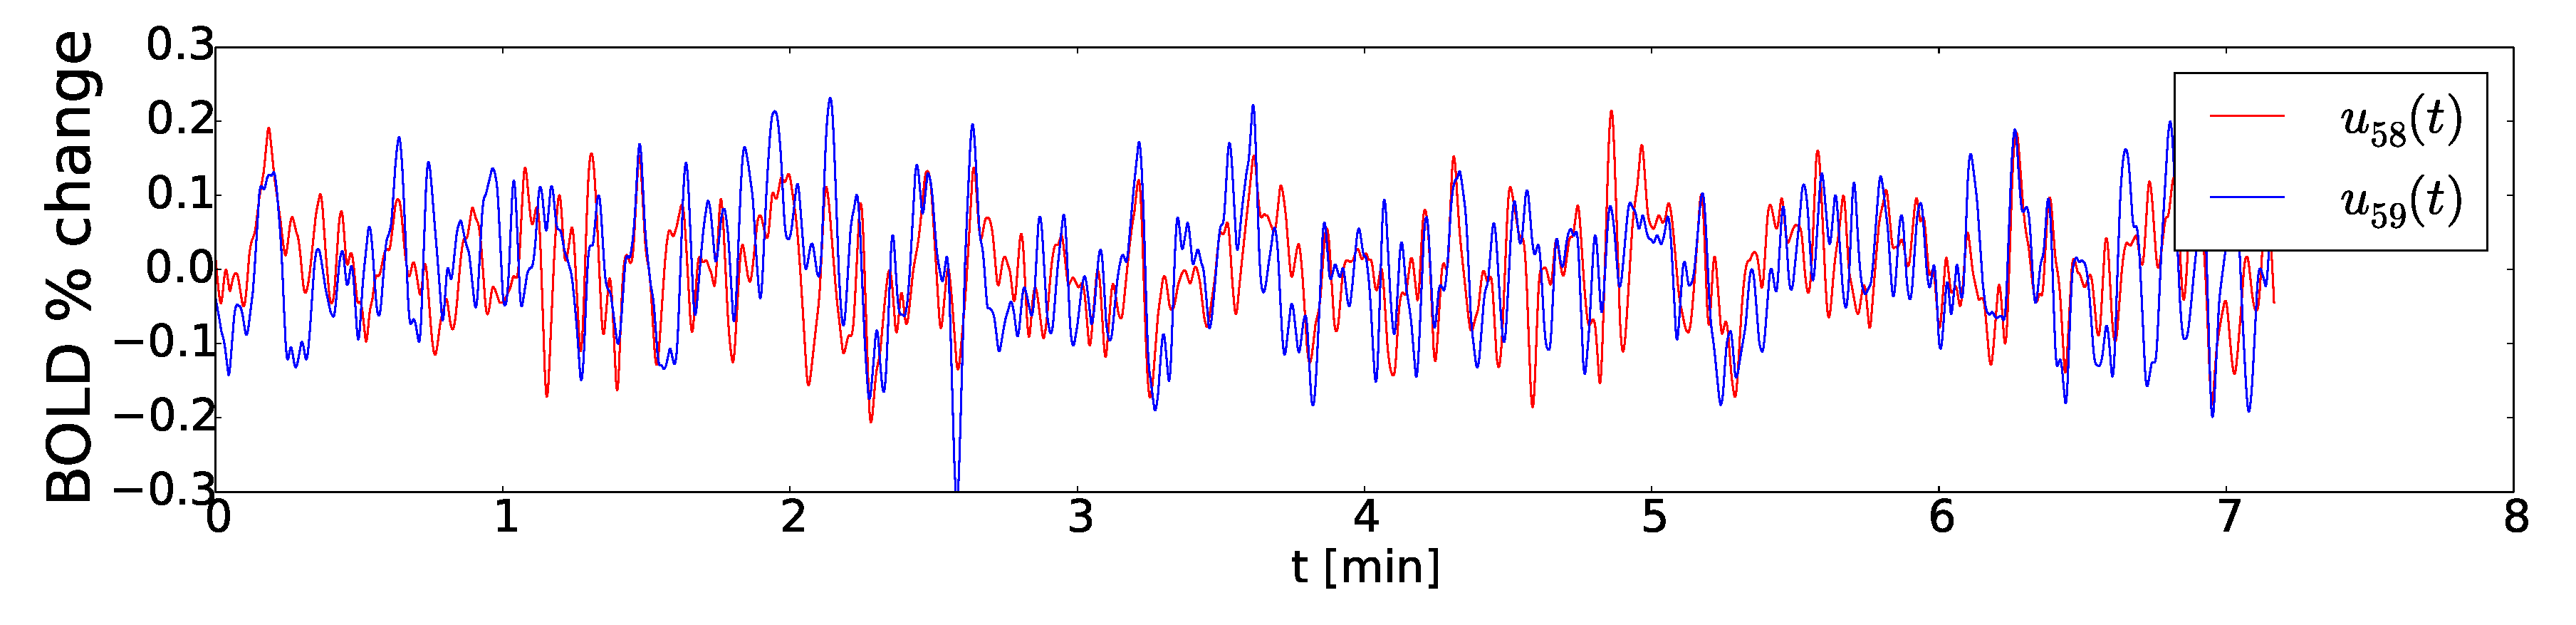
\includegraphics[width=\textwidth]{Figures/cor_BOLD_ACM_sim_no_best.eps} 
 
  \caption{Simulated BOLD activity of highly correlated node pairs with $\rho_{58,59}=0.48$. Both nodes are chosen from the FC$_s$ in Figure \ref{fig:BOLD_e_s} ($c=0.03$, $v=3$ m/s, $p=0.54$).} 
    \label{fig:BOLD_nodes}
\end{figure} 

Given a fast oscillating neuronal time-series as the input, the Ballon-Windkessel hemodynamic model acts on it as a low-pass filter \citep{FRI00}. The resulting BOLD fluctuations are ultra slow in the frequency range ($<$ 0.1 Hz). In terms of temporal dynamics here, we could produce the BOLD activity in this plausible frequency domain. Figure \ref{fig:BOLD_nodes} demonstrates temporal dynamics of the simulated BOLD activity of a node pair. This node couple is chosen from hot color parameters in the FC$_s$ in Figure \ref{fig:BOLD_e_s} to illustrate the synchronous nodal behavior. The extracted BOLD oscillations of nodes 58 (L, Frontal Mid Orb) and 59 (L, Gyrus Rectus) are synchronized with $\rho_{58,59}=0.48$. 


\subsection*{Temporal Dynamics of Brain Graph vs Random Graph}   

The AC map is binarized at probability values in $0.34 \leq p \leq 0.82$ range by amount of 0.04 step size. $R_{BG}$ and $R_{ER}$ is constructed at each $p$-value, then the neuronal activity as well as the BOLD fluctuations are modeled on each network. Figure \ref{fig:BG_vs_RG} compares simulated temporal dynamics of $R_{BG}$ and $R_{ER}$; for the FHN network model (left) and the Balloon-Windkessel model (right). These comparisons are quantified by Bhattacharya coefficients $d(H_{BG}, H_{ER})$ given by colorbars, where $H_{BG}$ and $H_{ER}$ refer to histogram distributions in $R_{BG}$ and $R_{ER}$, respectively. Here, the $H_{BG}$ and $H_{ER}$ are obtained by calculating $\rho_{i,j}$-values for the simulated time-series at specific $(p,c)$-values (see Figure \ref{fig:histo_ex}). 

In Figure \ref{fig:BG_vs_RG}, the hot colors indicate a diversity between $H_{BG}$ and $H_{ER}$, whereas the cold colors present an analogy. The FHN network modeled neuronal time-series of $R_{BG}$ can be clearly distinguished from that of $R_{ER}$ at $0.34 \leq p \leq 0.78 $ and at $0.015\leq c \leq 0.035$ in Figure \ref{fig:BG_vs_RG} (left). However, a clear pattern of diversity cannot be captured for the BOLD activity simulations between $R_{BG}$ and $R_{ER}$ (right).  

\begin{figure}[htp] \centering
	 \includegraphics[width=0.49\textwidth]{Figures/Random_ACM_PA_task.eps} 
	 \includegraphics[width=0.49\textwidth]{Figures/Random_bold_PA_task.eps} 
   	 \caption{The statistical comparison of brain graphs $R_{BG}$ and random graphs $R_{ER}$ in terms of their modeled temporal dynamics: FHN network model (left) and modeled BOLD activity (right). The heat map represents the degree of similarity between histogram distributions of simulated functional connectivity of $R_{BG}$ and $R_{ER}$; $d(H_{BG}, H_{ER})$. } 
    \label{fig:BG_vs_RG}
\end{figure} 


\begin{figure}[htp] \centering
	 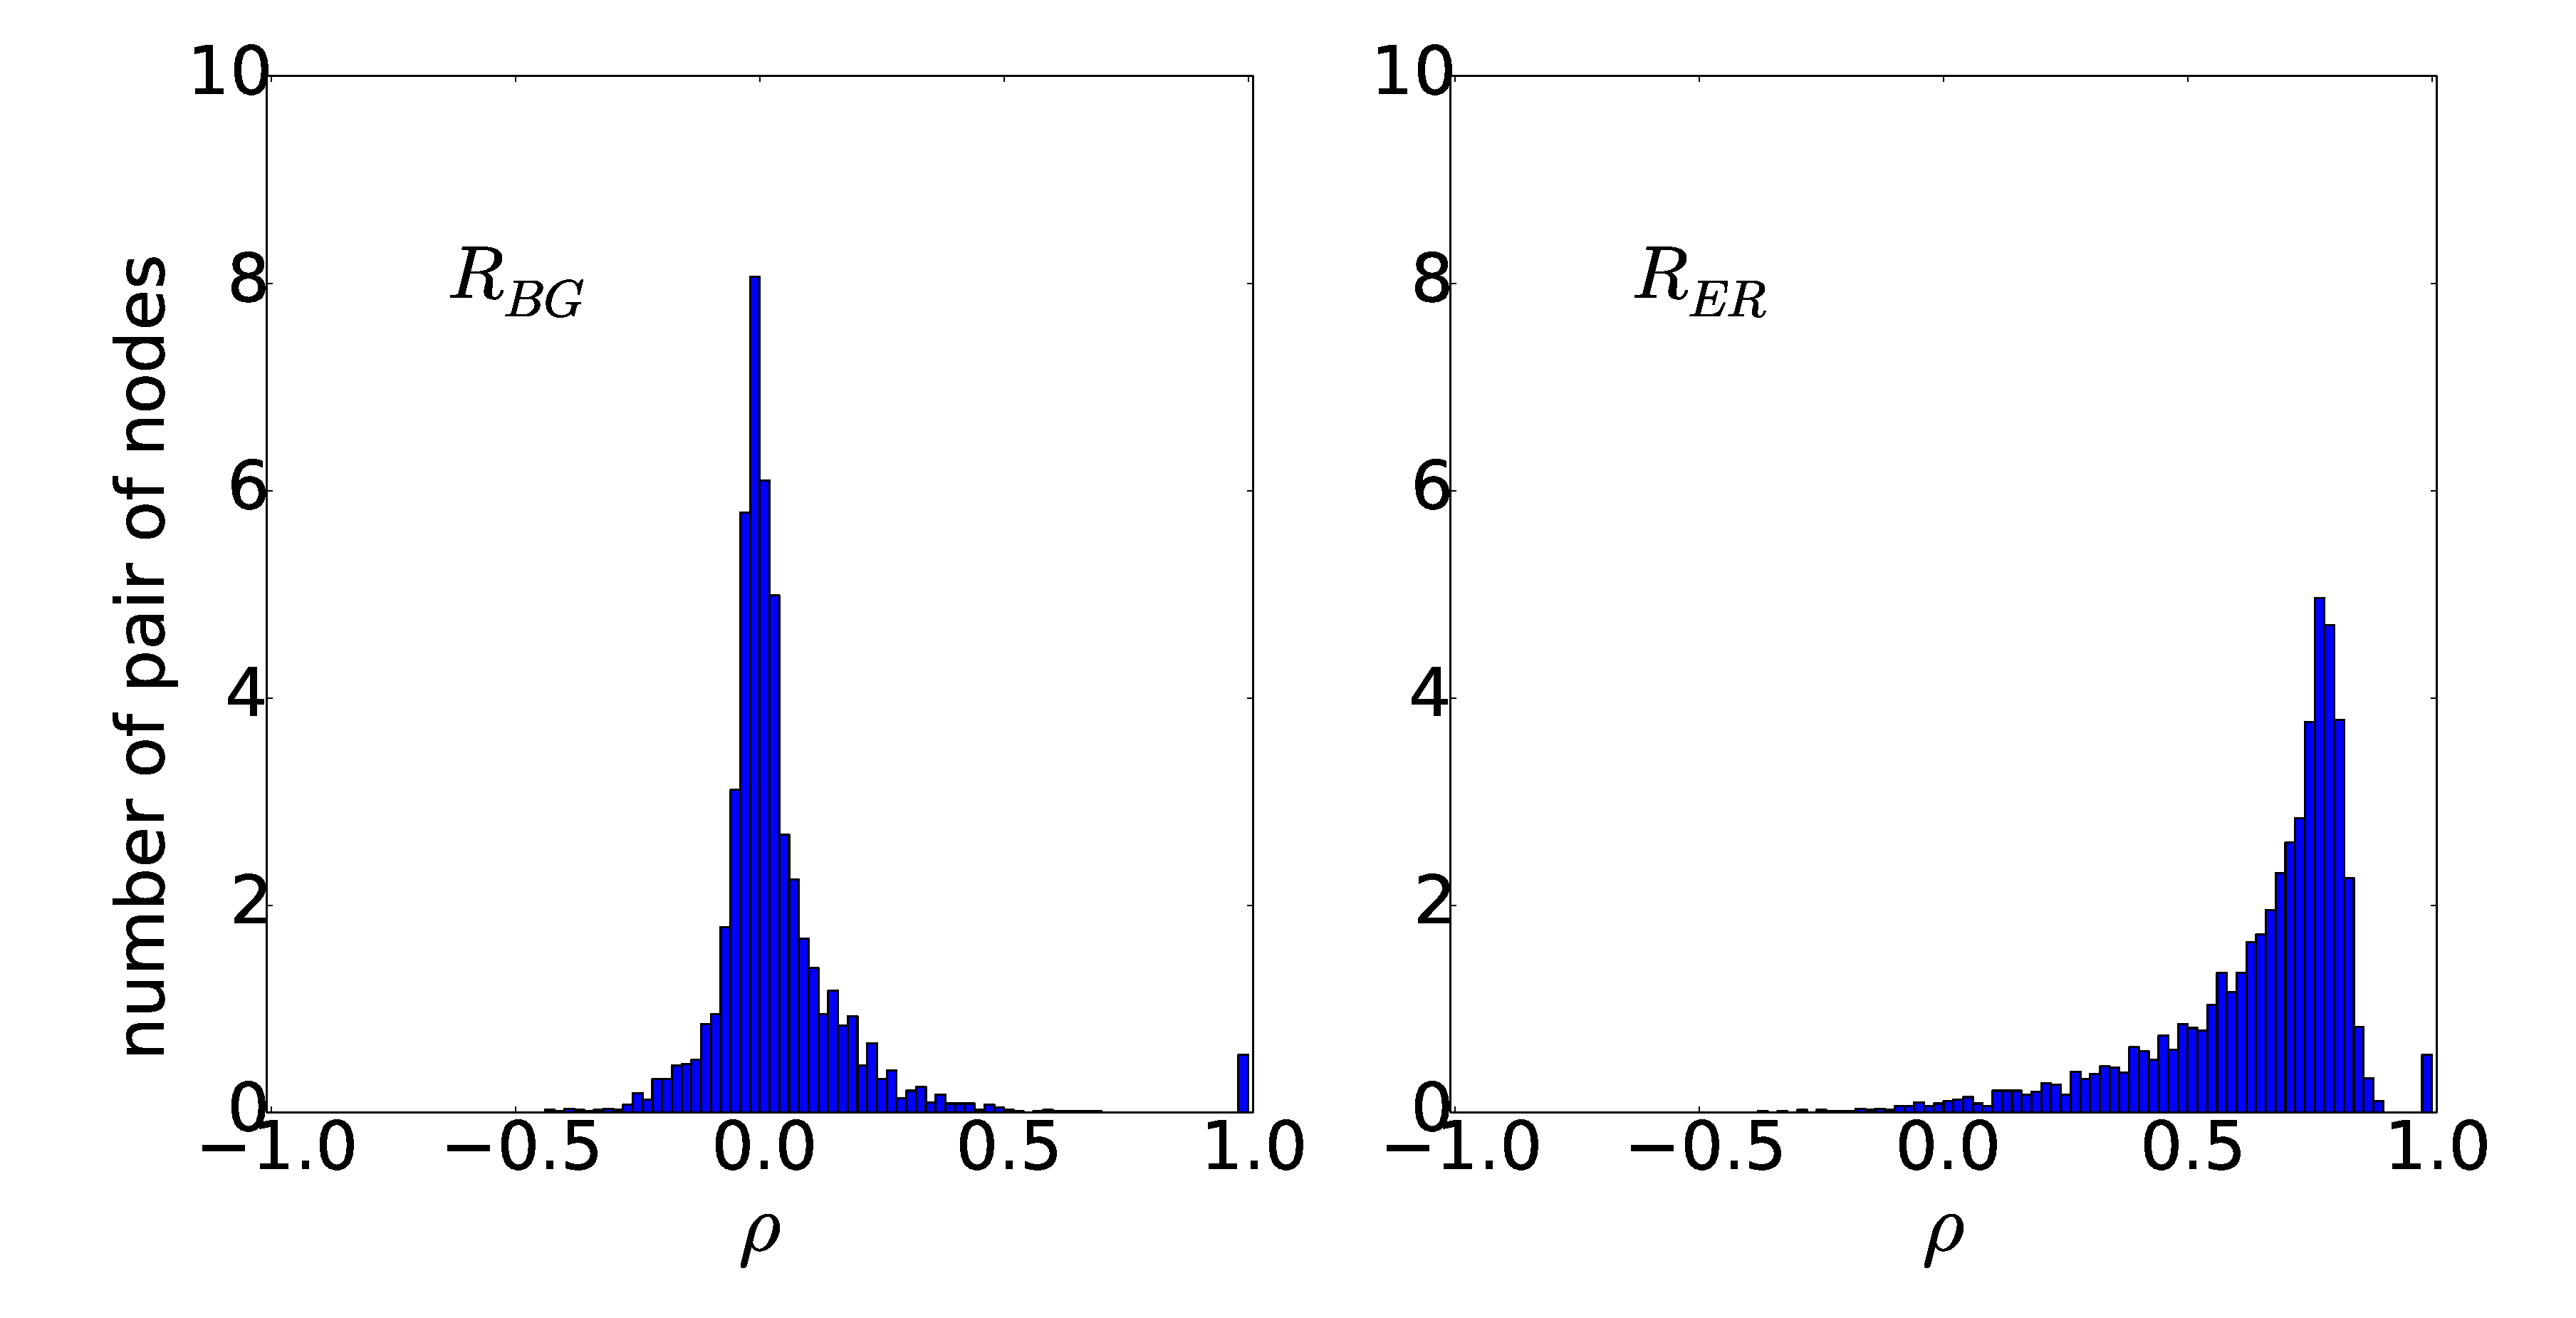
\includegraphics[width=0.85\textwidth]{Figures/Random_ACM_histo_taks.eps} 
   	 \caption{Histograms for the distribution of Pearson correlation coefficients $\rho$ among all possible pairwise combinations of nodal time-series in $R_{BG}$ (left) and $R_{ER}$ (right). The FHN network parameters for the chosen distributions are $c=0.03$ and $v=6$ m/s, the network topology parameter is $p=0.54$. } 
    \label{fig:histo_ex}
\end{figure} 

Figure \ref{fig:histo_ex} illustrates an exemplary set of histograms for the $R_{BG}$, which is constructed on an adjacency matrix obtained at $p=0.54$ given AC map, and for the $R_{ER}$, which is built by manipulating this adjacency matrix with Erd\H{o}s-R\'{e}nyi-type randomization tool. The frequency of $\rho$ values in $R_{BG}$ resembles a normal distribution around mean 0, indicating the dominance of non-correlated node pairs in terms of their FHN modeled time-series. However, $R_{ER}$ tends to have correlated time-series around $\rho=0.75$, and there seems to be almost no anti-correlation. The peaks at $\rho=1.0$ in each graph corresponds to self-paired nodes, i.e. $\rho_{i,i}=1.0$.  




\section*{Conclusion}

In this study, we simulated resting-state functional connectivity in human brain on structural and randomized networks. We showed that it is possible to capture traces of measured BOLD fluctuations by modeling the anatomical connectivity map. The BOLD signals arising from changing neuronal activity are affected by the anatomical connectivity in the cortex. We also addressed the topological characteristics of brain graphs, which are built on structural connectivity data, as well as random graphs, which are generated via manipulating these real graphs with Erd\H{o}s-R\'{e}nyi tool. Moreover, the analogy between brain and random networks are further analyzed by comparing their modeled temporal dynamics.  We demonstrated that the simulated neuronal time-series of brain graphs are clearly distinguishable than that of random networks at relatively low coupling strengths $c$ and reasonable connection probability ranges $p$.   


\section*{Acknowledgments}

This study was assisted by BMBF (grant no. 01Q1001B) in the framework of BCCN Berlin (Project B7). We would like to thank John-Dylan Haynes and his group for helpful discussions concerning the fMRI data analysis and Yasser Iturria-Medina for sharing the DTI data used in this work. \c{S}eyma Bayrak acknowledges additionally the support by Jochen Braun.





\bibliography{sample}

\newpage

\section*{Appendix}



\subsection*{Network Characterizations}

A network can be statistically described in terms of its topology, i.e. solely in terms of its connectivity and independently of spatial positions of nodes and edges. In this work, it is aimed to characterize the topology of $R_{BG}$ together with $R_{ER}$.   

\paragraph{Network Density}

The \textit{average degree} $\langle k \rangle$ of a network is proportional to the ratio of total number of edges $L$ to total number of nodes $N$ in a graph, 

\begin{equation}
\langle k \rangle = \frac{2L}{N}.
\end{equation}

The \textit{density} $\kappa$ of a network is formulated as the ratio between $L$ and maximum number of possible edges $\binom{N}{2}$,

\begin{equation}
\kappa = \frac{2L}{N(N-1)}.
\end{equation}	

The measure of network density can be referred to as the total \textit{wiring cost} of the network \citep{RUB10}. The \textit{degree} of an individual node $k_i$, average degree  $\langle k \rangle$ and network density $\kappa$ are key scalar measures to characterize the topology of a network. 

\paragraph{Average Clustering Coefficient}

The \textit{average clustering coefficient} $C$ of a network is calculated through individual clustering coefficients $C_i$ of single nodes,

\begin{equation}
C = \frac{1}{n} \sum\limits_{i\epsilon N}C_i = \frac{1}{n}\sum\limits_{i\epsilon N} \frac{2t_i}{k_i(k_i -1)} .
\end{equation} 

where $t_i$ is the number of triangles around node $i$ \citep{WAT98}. The clustering coefficient $C_i$ of a node $i$ is a measure of local connectivity and is highly correlated with the local efficiency of the information transfer \citep{LAT01}. The average clustering coefficient $C$ is a normalized version of $C_i$ for the whole network, yielding now a global property. $C$ is a measure of segregation, that is, the ability for specialized processing to occur within densely interconnected groups of brain regions \citep{RUB10}. It reveals how the individual nodes in a graph cluster together; how many neighbors of a node are neighbors of each other. 


\paragraph{Small-Worldness}

A small world network is both highly segregated and integrated, a measure of small worldness $S$ was proposed to capture this effect in a single statistic,

\begin{equation}
S = \frac{C/C_{rand}}{L/L_{rand}}, \,\,\,\,\,\,\,\,\,\,\,\,\,\,\,\,\,\,\,\,\,\,\,\,\,\,\,\,\,\,\,\,\,\,\,\,\,\,\,\, L = \frac{1}{n}\sum\limits_{i \epsilon N} L_i = \frac{1}{n}\sum\limits_{i \epsilon N} \frac{\sum\limits_{j \epsilon N, j \neq i }s_{ij}}{n-1 } \,\, .
\end{equation}
 
where $C$ and $C_{rand}$ are clustering coefficients, $L$ and $L_{rand}$ are characteristic path lengths of the original and random network respectively \citep{HUM08}. The random network here is constructed with \textit{Erd\H{o}s-R\'{e}nyi} method, which has the same number of nodes and links as the reference graph. $L$ is calculated through the shortest path length $s_{ij}$ between nodes $i$ and $j$, a basis for measuring integration \citep{RUB10}. 


\subsection*{Automated Anatomical Labeling}

Table \ref{tab:AAL} shows the Automated Anatomical Labeling (AAL) for the cortical and sub-cortical brain regions \citep{TZO02}. The brain is partitioned into $N=90$ regions symmetrically. AAL regions with index $n={1,2,...,45}$ lie on the right $R$ hemisphere, whereas $n={46,47,...,90}$ on the left $L$. The middle column of table describes the position of AAL regions anatomically in the cortex, and the last column corresponds to abbreviations.

\begin{table}[htbp] 
\centering
\caption[Automated Anatomical Labeling for the Brain Regions]{\label{tab:AAL}Anatomical Description of Brain Nodes }

\begin{tabular}{l | l | c}

Index R/L & Anatomical Description & Label \\ \hline  \hline 
  1/46 & Precentral & PRE   \\ 
  2/47 & Frontal Sup & F1 \\
3/48 & Frontal Sup Orb    &      F10 \\
4/49 & Frontal Mid        &       F2\\
5/50 & Frontal Mid Orb    &      F20\\
6/51 & Frontal Inf Oper   &    F30P\\
7/52 & Frontal Inf Tri    &     F3T\\
8/53 & Frontal Inf Orb    &      F30\\
9/54 & Rolandic Oper      &      RO\\
10/55 & Supp Motor Area  &      SMA\\
11/56 & Olfactory          &      OC\\
12/57 & Frontal Sup Medial  &   F1M\\
13/58 & Frontal Mid Orb     &   SMG\\
14/59 & Gyrus Rectus         &    GR\\
15/60 & Insula              &      IN\\
16/61 & Cingulum Ant       &   ACIN\\
17/62 & Cingulum Mid        &  MCIN\\
18/63 & Cingulum Post        & PCIN\\
19/64 & Hippocampus         &    HIP\\
20/65 & ParaHippocampal     &  PHIP\\
21/66 & Amygdala           &  AMYG\\
22/67 & Calcarine          &       V1\\
23/68 & Cuneus             &        Q\\
24/69 & Lingual            &   LING\\
25/70 & Occipital Sup      &       O1\\
26/71 & Occipital Mid      &       O2\\
27/72 & Occipital Inf      &       O3\\
28/73 & Fusiform           &    FUSI\\
29/74 & Postcentral        &   POST\\
30/75 & Parietal Sup       &       P1\\
31/76 & Parietal Inf       &       P2\\
32/77 & Supra Marginal Gyrus  &  SMG\\
33/78 & Angular               &   AG\\
34/79 & Precuneus             &   PQ\\
35/80 & Paracentral Lobule    & PCL\\
36/81 & Caudate               & CAM\\
37/82 & Putamen               & PUT\\
38/83 & Pallidum              &  PAL\\
39/84 & Thalamus              & THA\\
40/85 & Heschi                &  HES\\
41/86 & Temporal Sup          &    T1\\
42/87 & Temporal Pole sup     &  T1P\\
43/88 & Temporal Mid          &    T2\\
44/89 & Temporal Pole Mid     &  T2P\\
45/90 & Temporal Inf          &    T3\\
\hline  
  \hline 
                      
\end{tabular}
\end{table}


\end{document}